\chapter{Db2graph}
\label{chap:db2graph}

Im Rahmen dieses Kapitels wird IBM Db2graph genauer erläutert. Dabei wird der Ansatz, der Aufbau, die Funktionsweise und die bereits bekannten Einschränkungen der von Db2graph erläutert. 

\section{Ansatz}
\label{db2graph:ansatz}
Db2graph wurde mit dem Ziel entwickelt, Informationen mittels Graph-Queries aus einer relationalen Db2 Datenbank abfragen zu können. So wurde Db2graph als eine Art Graph-Erweiterung für Db2 konzipiert. Der Einsatz von Db2graph setzt folglich eine aktive Instanz von Db2 voraus \cite{vldb_tian, sigmod_tian}. Diese hält hierbei die Informationen, auf die Db2graph Zugriff hat, in relationaler Form \cite{vldb_tian, sigmod_tian}. Dabei müssen die Daten nicht für die Einbindung in Db2graph angepasst oder umformatiert werden \cite{vldb_tian, sigmod_tian}.

\begin{figure}[h]
    \centering
    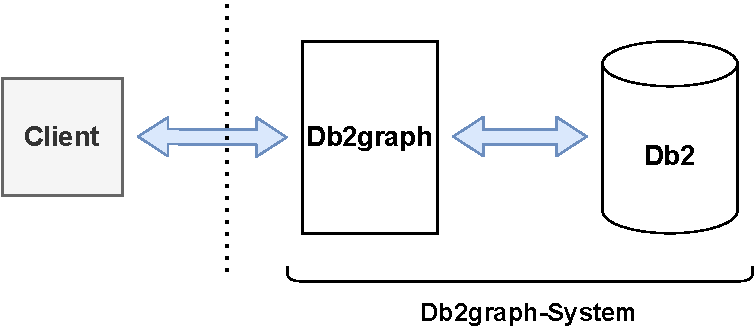
\includegraphics[width=\textwidth]{images/db2graph_system.pdf}
    \vspace{0.1em}
    \caption{Struktur Db2graph-System}
    \label{fig:db2graph_system}
\end{figure}

Wie in \autoref{fig:db2graph_system} erkennbar, fungiert Db2graph aus architektonischer Sicht als eine Art Proxy-Anwendung für Db2. Dabei übersetzt sie die von einem Client gesendeten Gremlin-Graph-Queries in SQL-An\-wei\-sung\-en und leitet diese anschließend an eine Db2 Instanz weiter \cite{vldb_tian, sigmod_tian}. Darüber hinaus können Db2 und Db2graph zusammengefasst als eine Art Hybrides Datenbankmanagementsystem betrachtet werden. Da es Elemente von Graph- und relationalen Datenbanksystemen vereint. So ist es möglich Graph-Anfragen an ein solches System zu stellen, während dem die Daten in relationaler Form gespeichert werden \cite{vldb_tian, sigmod_tian}. Im weiteren Verlauf der Arbeit wird die Kombination aus Db2 und Db2graph verkürzt als Db2graph-System bezeichnet, wie bereits in \autoref{fig:db2graph_system} dargestellt. 

\section{Aufbau}
Wie in \autoref{fig:db2graph_aufbau} beschrieben, handelt es sich bei Db2graph um eine modular aufgebaute Anwendung. Die Anwendung besteht dabei aus fünf größeren Komponenten. Die fünf Komponenten übernehmen dabei die folgenden Rollen und Aufgaben: 

\begin{itemize}
    \item \textbf{TinkerPop-Stack}\\Stellt das Grundgerüst für Db2graph dar. Er parst eingehende Gremlin-Queries und erstellt auf Basis dessen einen Query-Plan bzw. Abfrage-Plan \cite{vldb_tian}. Dabei interagiert er über API-Aufrufe mit den anderen Modulen \cite{vldb_tian}.
    \item \textbf{Topology}\\Beinhaltet die Funktionalität für das Mapping von relationalen Tabellen auf eine Graph-Struktur \cite{vldb_tian, sigmod_tian}.
    \item \textbf{Graph Structure}\\Hierbei handelt es sich um eine eigene Implementierung einer Graph-Struktur, auf deren Basis TinkerPop arbeitet \cite{vldb_tian}. Eine Implementierung dieser Struktur wird benötigt, um den vom TinkerPop-Stack erstellten Query-Plan durchzuführen \cite{sigmod_tian}. 
    \item \textbf{SQL-Dialect}\\Diese Komponente stellt die Funktionalität für die Erzeugung von Db2-kompatiblen SQL-Anweisungen bereit \cite{sigmod_tian}.
    \item \textbf{Traversal-Strategy}\\Dieses Modul stellt dem TinkerPop-Stack optimierte Traversal-Strategies zur Verfügung. Diese werden eingesetzt, um einen vom TinkerPop-Stack aufgestellten Query-Plan zu optimieren, bevor dieser ausgeführt wird \cite{sigmod_tian}.  
\end{itemize}

So stellt also der TinkerPop-Stack den Kern von Db2graph dar. Die Topology-, Graph-Structure- und SQL-Dialect-Komponente hingegen bieten Db2graph und Db2 spezifische Funktionalität, auf die der TinkerPop-Stack zugreifen kann. Das Traversal-Strategy-Modul stellt darüber hinaus dem TinkerPop-Stack, optimierte Traversal-Strategies zur Verfügung. Diese helfen dem TinkerPop-Stack dabei die Performance von Query-Plans zu verbessern.  

\begin{figure}[h]
    \centering
    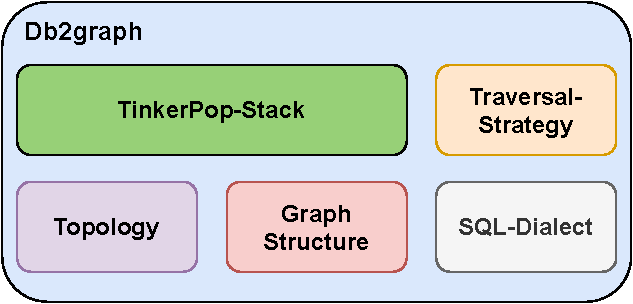
\includegraphics[width=\textwidth]{images/db2graph_components.pdf}
    \caption{Aufbau von Db2graph}
    \label{fig:db2graph_aufbau}
    \vspace{0.5em}
    \textit{Der hier gezeigter Aufbau von Db2graph   orientiert sich an der Beschreibung der System-Architektur in \cite{vldb_tian} und \cite{sigmod_tian}.}
\end{figure}

\section{Funktionsweise}
\label{db2graph:funktionsweise}
Um die Funktionsweise von Db2graph genauer zu erläutern, wird in diesem Abschnitt die Funktionsweise aus verschiedenen Perspektiven erläutert. Im Rahmen der ersten externen Perspektive wird detailliert darauf eingegangen, wie ein Db2graph-System die Anfrage eines Clients verarbeitet. Dabei wird erläutert, wie die Verarbeitung einer Gremlin-Query im Kontext einer Client-Anwendung, Db2graph und Db2 erfolgt. Bei der zweiten Perspektive handelt es sich hingegen um die Db2graph interne Perspektive. Im Zuge dessen wird beschrieben, wie eine Gremlin-Abfrage von einer Db2graph-Anwendung intern verarbeitet wird. Im Anschluss an diese beiden Perspektiven wird der Begriff und die Funktionsweise des Mapping in Db2graph genauer erläutert.

\subsection{Extern}
Die Funktionsweise beziehungsweise der Ablauf der Verarbeitung einer Graph-Query im Kontext eines Clients und Db2graph-Systems läuft wie folgt ab:

\begin{enumerate}
    \item Ein Client sendet eine Gremlin-Query an Db2graph. 
    \item Db2graph wandelt die Gremlin-Query in SQL-Statements um. 
    \item Db2graph sendet die erzeugten SQL-Statements an Db2.
    \item Db2 verarbeitet die SQL-Statements.
    \item Db2 leitet die Ergebnisse an Db2graph weiter.
    \item Db2graph bereitet die von Db2 empfangen Ergebnisse für den Client auf. 
    \item Db2graph übermittelt die Ergebnisse an den Client.
\end{enumerate}

Die soeben beschrieben Schritte des Ablaufs können dabei den in der \autoref{fig:db2graph_processing} aufgeführten Schritten zu geordnet werden. Die in \autoref{fig:db2graph_processing} als grün gekennzeichnet Pfeile markieren dabei die Schritte, in den die Anfrage in Form einer Gremlin-Query oder SQL-Anfragen weitergeleitet oder verarbeitet wird. Die Pfeile, welche in \autoref{fig:db2graph_processing} lila gefärbt sind, heben die Schritte hervor, in denen die abgefragten Daten transformiert oder weitergeleitet werden.

\begin{figure}[h]
    \centering
    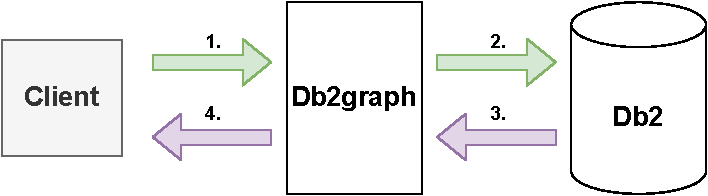
\includegraphics[width=\textwidth]{images/db2graph_processing.pdf}
    \caption{Externe Verarbeitung Db2graph}
    \label{fig:db2graph_processing}
    \vspace{1em}
    \textit{Die hier dargestellten Abläufe basieren hierbei unter anderem auf den in \cite{vldb_tian} und \cite{sigmod_tian} beschrieben Abläufen der Verarbeitung. Darüber hinaus wurden auch einige kleinere Details von \cite{tinkerpop_2020} bezogen.} 
\end{figure}

\subsection{Intern}
Im Rahmen dieses Unterabschnitts wird dargelegt, wie eine von Db2graph empfangene Gremlin-Query intern verarbeitet wird. Der Ablauf kann dabei in die folgenden Schritte gegliedert werden: 

\begin{enumerate}
    \item Ein Client baut Verbindung auf und sendet eine Gremlin-Query Db2graph.
    \item Der TinkerPop-Stack lädt Informationen über die Beschaffenheit des in der Gremlin-Query enthaltenen Zielgraphen aus Topology-Komponente \cite{vldb_tian,sigmod_tian, yt_tian}.
    \item Der TinkerPop-Stack erstellt auf Basis der Gremlin-Query und der Topologie-Informationen einen logischen Query-Plan auf \cite{vldb_tian,sigmod_tian, yt_tian}. 
    \item Der TinkerPop-Stack nutzt das Traversal-Strategy-Modul, um den logischen Query-Plan zu optimieren \cite{vldb_tian,sigmod_tian, yt_tian}.
    \item Der TinkerPop-Stack wandelt den optimierten logischen Query-Plan in einen physikalischen Query-Plan um \cite{vldb_tian,sigmod_tian, yt_tian}. 
    \item Bei der Ausführung der Steps im physikalischen Query-Plan werden API-Zugriffe auf die Graph-Structure-Komponente durchgeführt. Um die für diese Zugriffe benötigten Informationen zu beschaffen, lädt die Graph-Structure-Komponente Informationen aus dem Topology-Modul und nutzt die SQL-Dialect-Komponente für die Erzeugung von SQL-Statements. \cite{vldb_tian,sigmod_tian, yt_tian} 
    \item Die von der Graph-Structure-Komponente erzeugten SQL-Statements werden an eine Db2 Instanz gesendet und von dieser verarbeitet. \cite{vldb_tian,sigmod_tian, yt_tian}
    \item Die daraufhin von Db2 erhalten und zurückgesendeten Ergebnisse werden von der Graph-Structure-Komponente verarbeitet. \cite{yt_tian} 
    \item Die Graph-Komponente nutzt die verarbeiteten Ergebnisse, um die API-Aufrufe des TinkerPop-Stacks zu beantworten. \cite{vldb_tian,sigmod_tian, yt_tian} 
    \item Nach der Durchführung des physikalischen Query-Plans -- inklusive der API-Aufrufe auf die Graph-Structure-Komponente -- werden die Ergebnisse vom TinkerPop-Stack an den Client übermittelt \cite{vldb_tian,sigmod_tian, yt_tian}.
\end{enumerate}

Die in der zuvor aufgelisteten Schritten werden im Fall von 1. bis 7. auch nochmal in der \autoref{fig:db2graph_intern_processing} visuell dargestellt.

\begin{figure}[h]
    \centering
    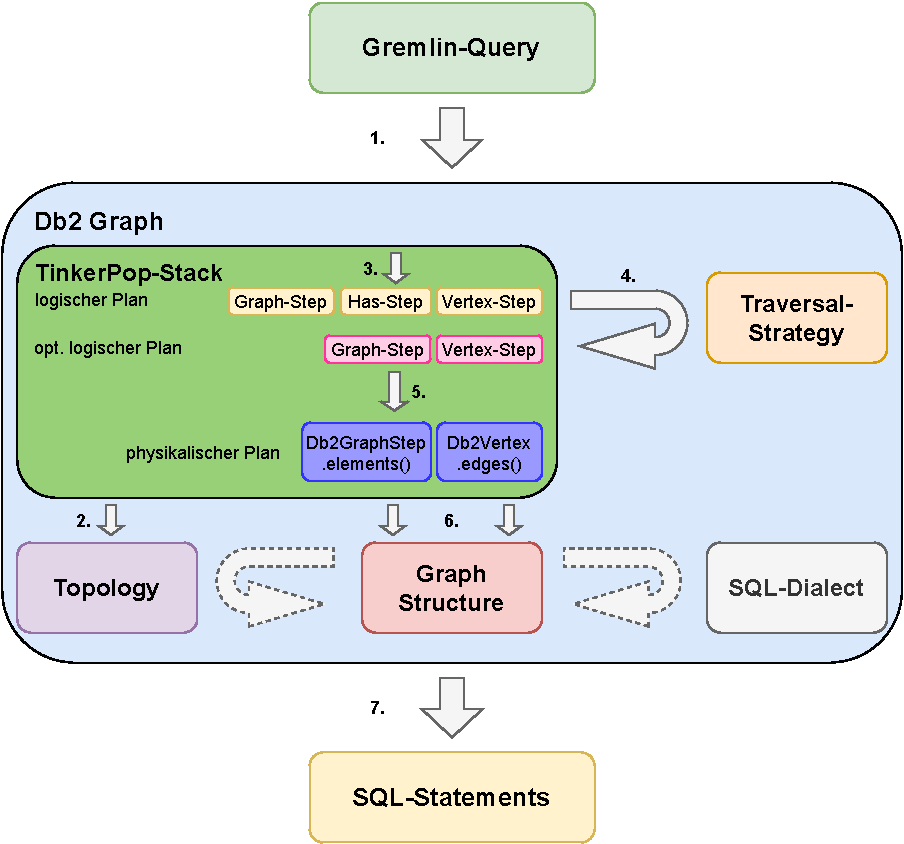
\includegraphics[width=\textwidth]{images/db2graph_intern_processing.pdf}
    \caption{Interne Verarbeitung Db2graph}
    \label{fig:db2graph_intern_processing}
    \vspace{1em}
    \textit{Die in der Abbildung dargestellten Abläufe basieren auf den in \cite{yt_tian}, \cite{vldb_tian} und \cite{sigmod_tian} beschrieben Abläufen.} 
\end{figure}

\subsection{Mapping}
Bei dem sogenannten Mapping handelt es sich um den Db2graph-internen Prozess beziehungsweise Technik, bei dem eine Graph-Struktur relationalen Daten überge\-stülpt wird beziehungsweise diese überlagert. Der Prozess kann auch als Graph-Overlaying bezeichnet werden. Im weiteren Rahmen der Arbeit wird der Prozess aber der Einfachheit halber als Mapping bezeichnet. Denn im Kern handelt es sich hierbei um ein Mapping von relationalen Tabellen und Spalten auf Graph-Elemente, wie Knoten und Kanten. Für die Bereitstellung und Verarbeitung des Mapping in Db2graph ist dabei die Topology-Komponente zuständig. 

Um das Mapping von relationalen auf Graph-Strukturen durchzuführen, werden den relationalen Tabellen verschiedene Rollen zugewiesen. Dabei sind die zwei folgenden Rollen verfügbar:
\begin{itemize}
    \item \textbf{VertexTable}\\Die Zeilen einer Tabelle werden als Knoten auf einen Graph gemappt \cite{sigmod_tian, yt_tian}.
    \item \textbf{EdgeTable}\\Die Zeilen dieser Tabelle werden als Kanten auf einen Graph gemappt \cite{sigmod_tian, yt_tian}.
\end{itemize}

Um Verbindungen zwischen Kanten und Knoten herzustellen  verfügt eine VertexTable über eine \texttt{vid}. Diese \texttt{vid} kann als eine Art Primärschlüssel betrachtet werden. Die \texttt{vid} setzt sich dabei aus einer oder mehreren Spalten einer relationalen Tabelle zusammen \cite{sigmod_tian, yt_tian}. Ihr Zweck ist es dabei, immer einen einzigen bestimmten Knoten über den Wert den \texttt{vid} identifizieren zu können \cite{sigmod_tian, yt_tian}. 

Auf Basis dieser \texttt{vid} setzt beim Mapping auch die EdgeTable auf. Um einen Quell- und Ziel-Knoten für eine Kante festzulegen, wird bei den EdgeTables angegeben, welche Spalten der Tabelle einen jeweiligen Quell- und Ziel-Knoten referenzieren. Dabei muss, um einen Verstoß gegen die referenzielle Integrität zu vermeiden, der Wert der \texttt{vid} dem Wert der referenzierten Spalten in der EdgeTable entsprechen. Darüber hinaus muss festgelegt werden, wie die  Namen der VertexTables lauten, die den Quell- und Ziel-Knoten einer Kante beinhalten. 

\section{Fähigkeiten \& Einschränkungen}

\section{Versionen}
